\label{chap:NoGANs}

Der Lernfortschritt von Klassifikatoren besteht darin, besser in der Aussage zu werden, ob ein Label $y$ auf einen gegebenen Eingang $x$ zutrifft. Dafür benötigen sie annotierte Trainingsdaten. Schachalgorithmen sollen hingegen lernen, Züge zu spielen, die die Gewinnchancen des Algorithmus maximieren. Eine weitere Art von \acp{KNN} sind \emph{generative Netze}. Sie sollen lernen, neue Daten zu erzeugen, die der Verteilung der Trainingsdaten ähneln. Generative Netze zur Bildgenerierung sollen demnach anhand eines Trainingsdatensatzes lernen, welche Bilder sie erzeugen sollen. Dies lernen sie anhand der statistischen Verteilung der Trainingsdaten. Die Daten sind nicht annotiert, wodurch generative Netze in der Regel in das \emph{Unüberwachte Lernen} einzuordnen sind.

\subsection{Mathematischer Hintergrund}
Generative Netze zur Bilderzeugung sollen beurteilen können, wie wahrscheinlich es ist, dass ein gegebenes Bild aus der Verteilung der Trainingsdaten stammt. Wenn $x$ für jedes mögliche existierende Bild steht, so bilden generative Netze folgende Wahrscheinlichkeitsverteilung ab:
\begin{equation}
   \hat{p}(x)
\end{equation}
Für ein gegebenes Bild $x$ gibt $\hat{p}(x)$ einen Schätzwert dafür an, wie wahrscheinlich es ist, dass das Bild aus den Trainingsdaten stammt. Diese Wahrscheinlichkeitsverteilung wird durch das Netz erlernt. Optimiert wird, dass die geschätzte Verteilung der Daten $\hat{p}(x)$ möglichst ähnlich zu der tatsächlichen Verteilung der Trainingsdaten $p(x)$ ist. Ein beispielhafter Vergleich ist in Abbildung \ref{fig:generativeNetsPx} dargestellt. Es ist erkennbar, dass sich die geschätzte und die tatsächliche Verteilung ähnlich sehen, jedoch nicht identisch sind. Die Abweichung zwischen diesen Verteilungen stellt dabei die Kosten (engl.: den \emph{loss}) dar. Die schwarzen Punkte kennzeichnen Trainingsdaten. Durch sie soll die Verteilung $p(x)$ abgebildet werden. Weniger diversifizierte Trainingsdaten würden sich beispielsweise nur in einem Teilbereich von $p(x)$ befinden. Dadurch könnte das Modell $p(x)$ weniger gut approximieren.

\begin{figure}[H]
   \centering
   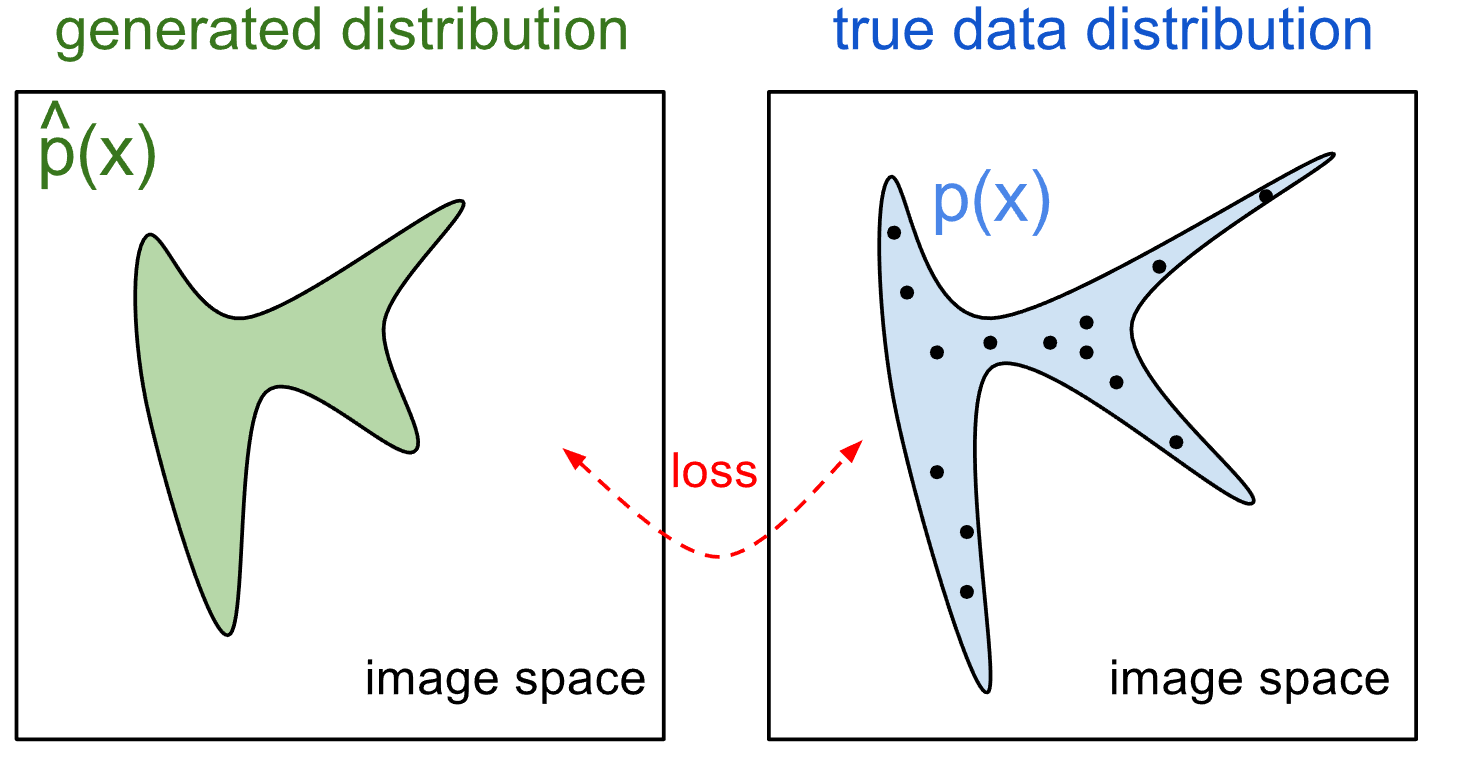
\includegraphics[width=0.5\textwidth]{images/Generative Networks/p(x) Distribution.png}
   \caption{Beispielhafter Vergleich von $\hat{p}(x)$ und $p(x)$ \cite{openAiGenerativeNets}}
   \label{fig:generativeNetsPx}
\end{figure}

Bei der Bildgenerierung versucht das Netz den Wahrscheinlichkeitswert für $\hat{p}(x)$ zu maximieren. Es erlernt durch $\hat{p}(x)$, wie die Verteilung der Trainingsdaten aussieht und versucht anschließend ausschließlich Bilder zu generieren, die dieser Verteilung folgen. Bezogen auf Abbildung \ref{fig:generativeNetsPx} befinden sich alle generierten Bilder des trainierten Netzes im grün markierten Bereich.

Es existieren verschiedene Arten generativer Netze. Die Taxonomie, also die Einteilung verschiedener Netze in bestimmte Kategorien, kann Abbildung \ref{fig:generativeModelsTaxonomy} entnommen werden. Einerseits existieren Architekturen, die die Wahrscheinlichkeitsverteilung $\hat{p}(x)$ explizit berechnen. Andere berechnen die Funktion nicht, verwenden sie jedoch implizit. In der Abbildung wird dahingehend zwischen \emph{Explicit Density Models} \emph{(explizit berechnete Dichte)} und \emph{Implicit Density Models} \emph{(implizit berechnete Dichte)} unterschieden. Es existieren zudem Unterkategorien, mittels derer eine feinere Kategorisierung durchgeführt wird.

\begin{figure}[H]
   \centering
   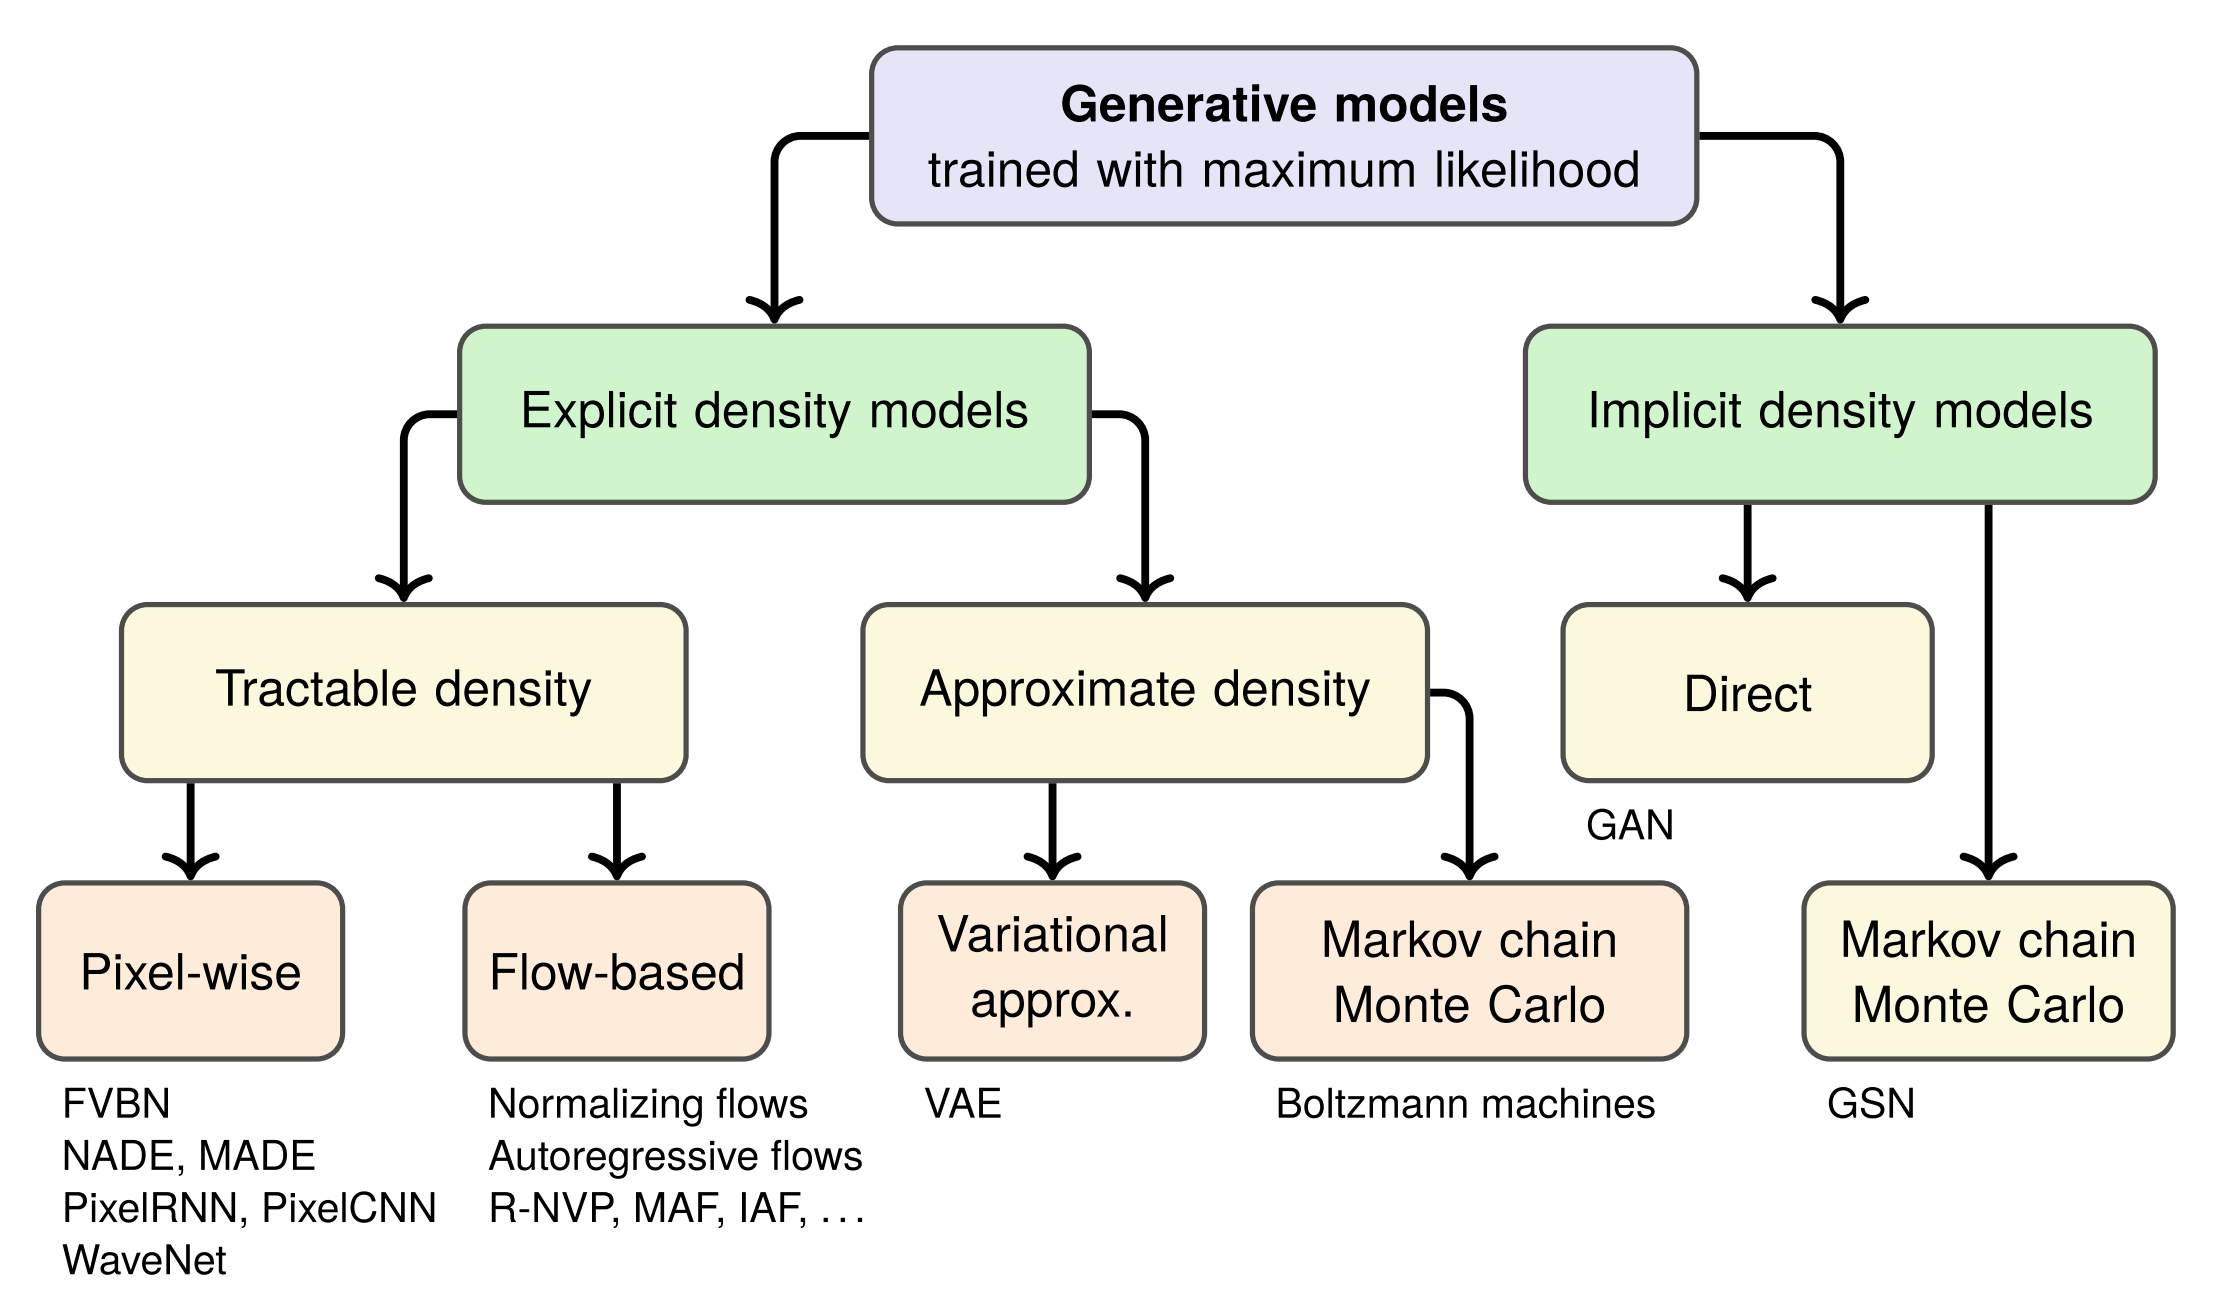
\includegraphics[width=0.8\textwidth]{images/Generative Networks/Taxonomy of Generative Models.png}
   \caption{Taxonomie generativer Modelle \cite{generativeModelsBook}}
   \label{fig:generativeModelsTaxonomy}
\end{figure}

Es soll in diesem Kapitel auf verschiene Architekturen generativer Netze eingegangen werden. \acp{GAN} werden gesondert in Kapitel \ref{chap:GANs} beschrieben.

\subsection{Pixel Recurrent Neural Networks}
Die Architektur der \acp{PixelRNN} stammt aus dem Jahr 2016. Diese Netze stützen sich explizit auf die Maximierung der Maximum-Likelihood-Schätzung von $\hat{p}(x)$ für jeden Pixel. Sie sind in der genannten Taxonomie den Modellen zuzuordnen, die den tatsächlichen Schätzwert von $p(x)$ berechnen können. \cite{pixelRNN}

Im folgenden soll geklärt werden, wie der optimale Wert für jeden Pixel eines generierten Bildes bestimmt wird. Ein betrachtetes Bild $x$ der Auflösung $n \times n$ kann in seine einzelnen Pixel $(x_{1}, x_{2}, ..., x_{n^2})$ aufgeteilt werden. In Gleichung \ref{eq-max-likelihood} ist dabei dargestellt, wie die Wahrscheinlichkeit eines jeden Pixels in die gesamte Verteilung $\hat{p}(x)$ einfließt. \cite{pixelRNN}
\begin{equation}
   \label{eq-max-likelihood}
   \hat{p}(x) = \hat{p}(x_{1}, x_{2}, ..., x_{n^2}) = \prod_{i=1}^{n^2}\hat{p}(x_{i}|x_{1},...,x_{i-1})
\end{equation}
Jeder Pixel $x_{i}$ besitzt eine eigene Wahrscheinlichkeitsverteilung $\hat{p}(x_{i}|x_{1},...,x_{i-1})$. Sie ist abhängig von allen anderen Pixeln $x_{1},...,x_{i-1}$ des Bildes. Der absolut optimale Wert eines Pixels kann demnach nur dann berechnet werden, wenn die Werte aller anderen Pixel bekannt sind. Das Produkt aller Wahrscheinlichkeitswerte der einzelnen Pixel ergibt $\hat{p}(x)$. Soll $\hat{p}(x)$ maximiert werden, so müssen die Terme $\hat{p}(x_{i}|x_{1},...,x_{i-1})$ möglichst hohe Werte liefern. Daraus ergibt sich dann unter gegebenem Kontext für jeden Pixel eine Maximum-Likelihood-Schätzung. Also der Wert, für den $\hat{p}(x)$ möglichst weit gegen \emph{eins} strebt. \cite{pixelRNN}

Die Idee von PixelRNNs ist, dass bei der Generierung in einer Ecke des Bildes gestartet wird. Das Bild wird zunächst auf einen Pixel reduziert, der im folgenden $x_{1}$ genannt wird. Für diesen Pixel wird ein Wert generiert. Anschließend wird $x_{1}$ gemeinsam mit einem benachbarten Pixel $x_{2}$ betrachtet. Die Wahrscheinlichkeitsverteilung für $x_{2}$ ergibt sich dadurch zu $\hat{p}(x_{2}|x_{1})$. Der Wert für $x_2$ ist somit nur von $x_1$ abhängig. Da $x_{1}$ bekannt ist, kann ein optimaler Wert für $x_{2}$ bestimmt werden. Die Wahrscheinlichkeitsverteilung von $x_{3}$ ergibt sich zu $\hat{p}(x_{3}|x_{1}, x_{2})$, die von $x_{4}$ zu $\hat{p}(x_{4}|x_{1}, x_{2}, x_{3})$. Das Bild wird sukzessive generiert, wobei der momentane Pixelwert für $x_{i}$ von allen bisher generierten Pixeln abhängig ist. Dieses vorgehen ist in Abbildung \ref{fig:pixelRNN} dargestellt. Der Wert des rot markierten Pixels hängt von allen blau markierten Pixel ab. Ist für diesen ein Wert bestimmt, wird der rechtsseitig benachbarte Pixel als neues $x_{i}$ gewählt.

\begin{figure}[H]
   \centering
   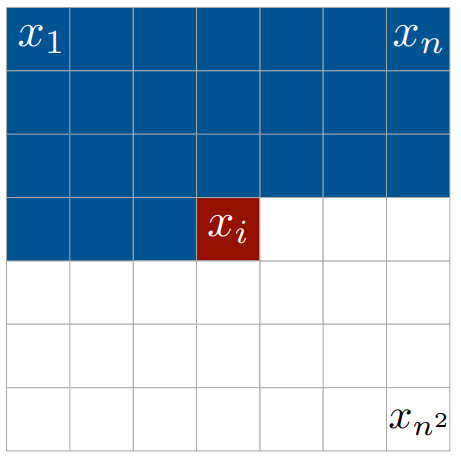
\includegraphics[width=0.25\textwidth]{images/Generative Networks/PixelRNN.png}
   \caption{Bestimmung von $\hat{p}(x)$ mit PixelRNNs \cite{pixelRNN}}
   \label{fig:pixelRNN}
\end{figure}

Um die beschriebene Abhängigkeit des momentan generierten Pixels zu allen bisher generierten Pixel umsetzen zu können, besitzen \acp{PixelRNN} eine Art \emph{Erinnerung}. Bisher wurden in dieser Arbeit nur sogenannte \emph{Feedforward} Netze behandelt, bei denen der Informationsfluss stets in eine Richtung erfolgt. Nämlich vom Eingang des Netzes zum Ausgang. Es existieren auch \emph{Recurrent Neural Networks}. Sie werden besonders zur Verarbeitung von natürlicher Sprache eingesetzt \emph(engl.: natural language processing). Abbildung \ref{fig:RNN} bildet hierfür eine beispielhafte Darstellung.

\begin{figure}[H]
   \centering
   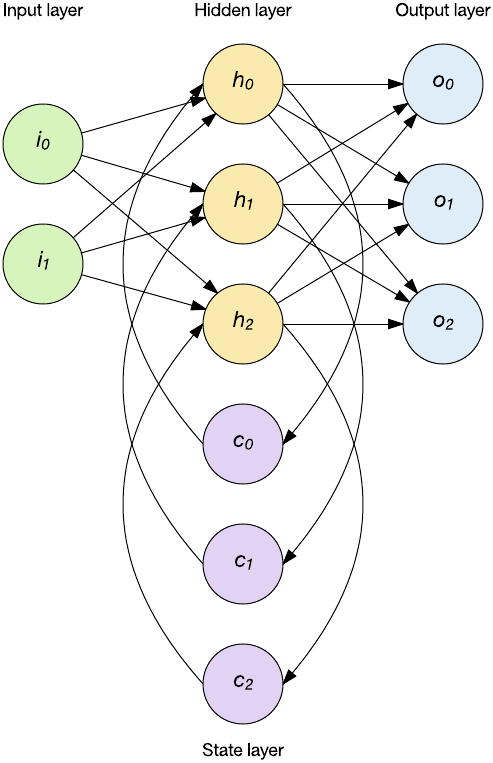
\includegraphics[width=0.375\textwidth]{images/Generative Networks/RNN.png}
   \caption{Darstellung eines Recurrent Neural Networks \cite{ibmRNN}}
   \label{fig:RNN}
\end{figure}

In Recurrent Neural Networks spielen die \emph{Zustände} eines Netzes eine besondere Rolle. Ein Zustand wird durch die Eingangs- und Ausgangswerte aller Neuronen zu einem gegebenen Zeitpunkt beschrieben. In \acp{PixelRNN} ist der Zustand des Netzes für den Pixel $x_{2}$ abhängig von dem Zustand des Netzes für $x_{1}$. Um solche Beziehungen darstellen zu können, besitzt das beispielhaft abgebildete Netz die Neuronen $c_{0}$ bis $c_{2}$, die den vorherigen Wert eines Neurons rekursiv auf seinen Eingang zurückführen. Somit wird der vorherige Zustand des neuronalen Netzes als zusätzlicher Eingang für die Berechnungen genutzt. \acp{PixelRNN} nutzen eine besondere Form der Recurrent Neural Networks. Sie arbeiten mit sogenannter \emph{Long Short-term Memory}. Dadurch soll das Problem behoben werden, dass in klassischen Recurrent Neural Networks weit in der Vergangenheit liegende Zustände nur noch einen geringen Einfluss auf den momentanen Zustand haben. \cite{generativeModelsSurvey}

Da die durch ein \ac{PixelRNN} umgesetzte Verteilung $\hat{p}(x)$ direkt erfassbar ist, wird ihnen nachgesagt, dass die Performanz solcher Netze gut evaluiert werden kann. Es gilt als vergleichsweise leicht, für solche Netze Metriken zur Messung der Performanz umzusetzen. Ein grundlegender Nachteil von \acp{PixelRNN} ist, dass die Generierung sequenziell erfolgt. Es ist in dem beschriebenen Verfahren nicht möglich, mehrere Pixel parallel zu generieren, da der Wert eines Pixels von denen aller vorher generierten Pixel abhängig ist. Dies verlangsamt die Generierung, da keine Parallelisierung möglich ist. \cite{generativeModelsSurvey}

Es existieren auch sogenannte \emph{PixelCNNs}, bei denen sich die Berechnung stets nur auf bestimmte Bildbereiche konzentriert. Diese Bildbereiche können parallel zueinander sequenziell berechnet werden. Die Parallelisierung ist jedoch nur während des Trainings des Netzwerks oder während der Evaluation von $\hat{p}(x)$ für gegebene Bilder möglich. Die Bildgenerierung erfolgt auch hier, analog zu \acp{PixelRNN}, vollständig sequenziell. \cite{pixelRNN}

\subsection{Autoencoder}

Das Ziel von Autoencodern ist, den Eingang des Netzes am Ausgang zu rekonstruieren. Dazu setzen sich diese Netze aus drei Bestandteilen zusammen: dem Kodierer, dem latenten Raum und dem Dekodierer. In Abbildung \ref{fig:Autoencoder} ist eine beispielhafte Autoencoderarchitektur dargestellt.

\begin{figure}[H]
   \centering
   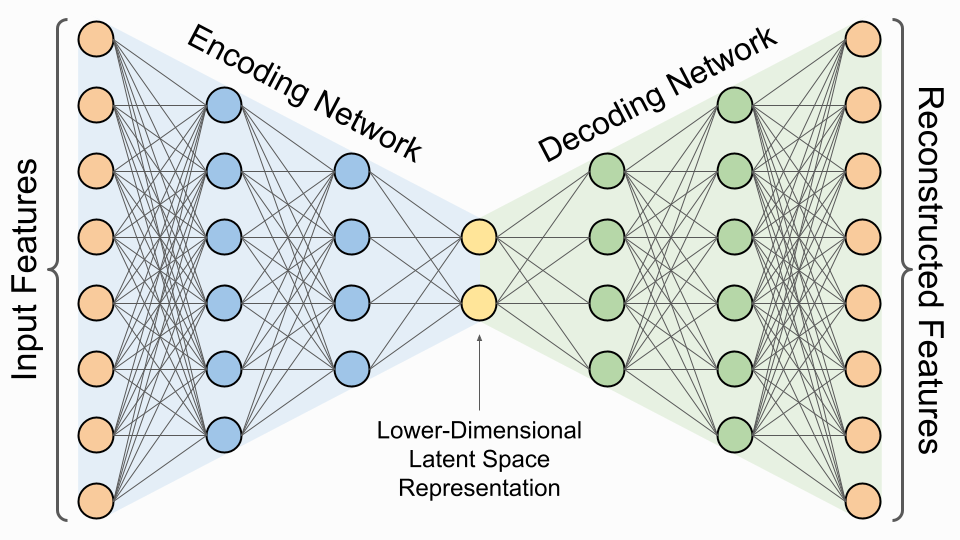
\includegraphics[width=0.65\textwidth]{images/Generative Networks/autoencoder_architecture.png}
   \caption{Architektur eines Autoencoders}
   \label{fig:Autoencoder}
\end{figure}

Der \textbf{Kodierer} besitzt die Aufgabe, Merkmale aus dem Eingang des Netzes zu extrahieren. Diese Merkmale sollen daraufhin mit einer begrenzten Anzahl an Parametern durch den latenten Raum repäsentiert werden. Somit besteht die Aufgabe des Kodierers darin, den Eingang auf seine für das Netz wesentlichen Eigenschaften zu reduzieren. Und zwar erfolgt die Komprimierung dabei so, dass die Informationen gerade so durch den latenten Raum dargestellt werden können. 

Bei dem \textbf{latenten Raum} handelt es sich um eine einzelne Schicht von Parametern, oder in diesem Kontext: Neuronen. Je mehr Neuronen sich in dem latenten Raum befinden, desto mehr Informationen können von der Kodierung an die Dekodierung übertragen werden. Die Merkmale, die sich in dem latenden Raum befinden, können durch einen Vektor $\vec{z}$ beschrieben werden. Der latente Raum sollte klein genug sein, damit dort nicht alle Merkmale des Eingangs gespeichert werden können. So wird der Kodierer dazu gezwungen, vereinzeilte Merkmale zu extrahieren. 

Der \textbf{Dekodierer} nutzt die Werte aus dem latenten Raum, um den Eingang nachzubilden. Diese Nachbildung stellt den Ausgang des Autoencoders dar. Die Kosten eines Autoencoders können durch die Abweichung zwischen Ein- und Ausgang festgestellt werden. 

Da der Zweck von Autoencodern darin besteht, einen Eingang auf seine relevanten Merkmale zu reduzieren, wird der Dekodierer nur während des Trainings verwendet. Beim praktischen Einsatz eines Autoencoders werden lediglich der Kodierer und der latente Raum eingesetzt. Im Gegensatz zu \acp{PixelRNN} basieren Autoencoder klassischerweise nicht auf Recurrent Neural Networks, sondern auf Feedforward Netzen.

Diese beschriebene Architektur der Autoencoder ist nicht für die generative Modellierung geeignet, da sie deterministisch ist. Erhält das Modell bestimmte Eingangswerte, so liefert es stets die gleichen Ausgangswerte. Es versucht den Eingang möglichst zu rekonstruieren, wobei der Inhalt $\vec{z}$ des latenten Raums für ein gegebenes Eingangsbild stets gleich ist. Eine zufällige Erzeugung neuer Bilder ist damit nicht möglich. Die sogenannten \emph{Variational Autoencoder} sind eine Architektur, die für die Generierung neuer Daten verwendet werden können. \cite{visualApproach}

\textbf{Variational Autoencoder} verfolgen das Ziel, eine Zufallskomponente in die Bilderzeugung einfließen zu lassen. Ein entscheidender Unterschied zu klassischen Autoencodern ist deshalb der folgende: Ein gegebener Eingang $x$ wird auf kein festes $\vec{z}$ kodiert, sondern auf eine Wahrscheinlichkeitsverteilung. Sie wird bezeichnet als:
\begin{equation}
   p(z|x)
\end{equation}
Im Gegensatz zu \acp{PixelRNN} versucht das Netz somit nicht die Verteilung der Trainingsdaten $p(x)$ zu approximieren, sondern die Verteilung der Merkmale $\vec{z}$ der Trainingsdaten $x$.
Es wird angenommen, dass jedes Merkmal normalverteilt ist. Damit kann jede Komponente $z_{i}$ des Vektors $\vec{z} = [z_{1}, z_{2}, ..., z_{n}]^\mathsf{T}$ durch eine Gaußsche Normalverteilung $\mathcal{N}(\mu_{i}, {\sigma_{i}}^{2})$ beschrieben werden. Aufgabe des Kodierers ist damit nicht mehr, aus einem gegebenen $x$ eine Menge von Merkmalen $\vec{z}$ zu bestimmen. Stattdessen soll der Kodierer die Vektoren $\vec{\mu}$ und $\vec{\sigma}$ bestimmen, durch die sich die einzelnen Normalerteilungen von $\vec{z}$ beschreiben lassen. 

An den Dekodierer wird ein zufällig aus der Verteilung $p(z|x)$ entnommenes Set an Merkmalen $\vec{z}$ übergeben.
Der Dekodierer übersetzt dieses gegebene $\vec{z}$ daraufhin in ein Bild. Im praktischen Einsatz werden bei einem Variational Autoencoder nur der latente Raum und der Dekodierer genutzt. Der Dekodierer erhält zufällige Werte für $\vec{z}$, also zufällige Merkmale, und generiert daraus ein Bild.

\textbf{Vor- Nachteile?}

\cite{autoencoders}

\label{chap:GANs}
\subsection{Generative Adversarial Networks}
Eine weitere Architektur, die zur Bildgenerierung verwendet werden kann, sind die sogenannten \emph{Generative Adversarial Networks} (\acsp{GAN}). Sie wurden unter anderem von Ian Goodfellow im Jahre 2014 entwickelt.

Ein \ac{GAN} besteht aus zwei Komponenten. Dem \emph{Generator} und dem \emph{Discriminator}.
Der Generator erzeugt aus einem zufälligen Eingangsvektor ein Bild. Der Discriminator erhält ein Bild als Eingang und gibt entweder den Wert \emph{0} oder den Wert \emph{1} aus. Er soll erkennen, ob das gegebene Bild aus den Trainingsdaten stammt, oder ob es künstlich generiert wurde. Bei sowohl dem Generator als auch dem Discriminator handelt es sich um \acp{KNN}. Diese beiden Komponenten werden so miteinander gekoppelt, dass der Discriminator stets entweder ein erzeugtes Bild des Generators oder ein Bild aus den Trainingsdaten erhält. Dies ist in der nachfolgenden Abbildung beispielhaft dargestellt:
\begin{figure}[H]
	\centering
	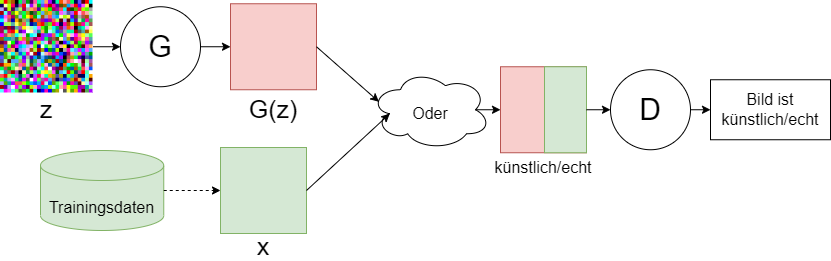
\includegraphics[width=0.8\textwidth]{../images/GANs/GAN.drawio.png}
	\caption{Zusammenspiel zwischen Generator und Discriminator}
	\label{fig:gan}
\end{figure}
Der Generator G erhält einen zufälligen Eingangsvektor $z$. Letzterer kann als ein weißes Rauschen beschrieben werden. Das generierte Bild ist das Resultat der Funktion $G(z)$ des Generators G. Anschließend wird dem Discriminator D entweder das generierte Bild $G(z)$ oder ein Bild $x$ aus den Trainingsdaten gezeigt. Der Ausganswert des Discriminators ist daraufhin die Einschätzung, ob das gezeigte Bild echt oder künstlich generiert ist. Ziel des Generators ist, dass die Verteilung der künstlichen Daten $p(G(z))$ möglichst ähnlich der Verteilung $p(x)$ ist. Der Discriminator soll die beiden Verteilungen möglichst gut voneinander unterscheiden können. Somit handelt es sich um ein direktes Gegenspiel zwischen Generator und Discriminator. Sie versuchen sich gegenseitig zu überlisten.

\paragraph{Training}
Dies spiegelt sich auch im Training von \acp{GAN} wider. $V(D,G)$ stellt die zu optimierende Funktion dar: \cite{Goodfellow-GANs}
\begin{equation}
   \label{eq:adv_loss}
	\min_{G} \max_{D} V(D,G) = \mathbb{E}_{x}[\log(D(x))] + \mathbb{E}_{z}[\log(1-D(G(z)))]
\end{equation}
Bei dem Training handelt es sich um ein Min-Max-Problem. Der Generator versucht die Funktion $V(G,D)$ zu minimieren, wohingegen der Discriminator sie zu maximieren versucht. Der Term \ref{eq:real_adv_loss} stellt die Fehlerrate des Discriminators auf den echten Trainingsdaten dar. Mit anderen Worten: Wie viele echte Bilder er als unecht klassifiziert. Der Term \ref{eq:fake_adv_loss} beschreibt, wie viele unechte Daten der Discriminator als echt klassifiziert. \cite{visualApproach}
\begin{equation}
   \label{eq:real_adv_loss}
	\mathbb{E}_{x}[\log(D(x))]
\end{equation}
\begin{equation}
   \label{eq:fake_adv_loss}
	\mathbb{E}_{z}[\log(1-D(G(z)))]
\end{equation}
Der Term \ref{eq:real_adv_loss} ist nicht vom Generator abhängig, sondern lediglich von $D(x)$. Hierauf hat der Generator keinen Einfluss, wodurch er alleine durch diesen Teil der Kostenfunktion nicht trainiert wird. Der Discriminator besitzt somit zwei Terme, die ihn trainieren, während der Generator nur einen besitzt. Aus diesem Grund werden dem Discriminator in der Regel doppelt so viele unechte Daten wie echte Trainingsdaten gezeigt. Dies soll einem ungleichen Training der beiden Komponenten des \acp{GAN} entgegenwirken. Der Optimalzustand eines \acp{GAN} ist, dass der Discriminator so gut wie möglich identifizieren kann, ob ein gegebenes Bild aus $p(x)$ stammt, während der Generator dennoch in der Lage ist, den Discriminator zu überlisten. Das Training von \acp{GAN} gilt als empfindlich gegenüber den gewählten Hyperparametern und der Netzwerkarchitektur. \acp{GAN} wird nachgesagt, dass kleine Änderungen in den beiden genannten Aspekten die Qualität der Generierten Bildern signifikant beeinflussen können. \cite{visualApproach}

Im praktischen Einsatz wird nur der Generator des \acp{GAN} verwendet. Der Discriminator wird ausschließlich dazu eingesetzt, mit $p(G(z))$ möglichst gut $p(x)$ zu approximieren, sodass die generierten Bilder im Optimalfall nicht von echten Trainingsdaten zu unterscheiden sind. \cite{visualApproach}
%Analog zu Kapitel \ref{chap:NoGANs}, ist die Aufgabe des Generators, Daten aus der Wahrscheinlichkeitsverteilung $p(x)$ der Trainingsdaten zu erzeugen. Der Eingangsvektor $z$ des Generators folgt einer Verteilung $p_z(z)$. Der Generator kann durch folgende Funktion beschrieben werden:

%\begin{equation}
%	G(z, \theta_{g})
%\end{equation}

%Der Generator erzeugt neue Bilder, während der Discriminator für jedes erzeugte Bild rät, ob es aus dem Trainingssatz stammt, oder ob es künstlich generiert ist. Nur der Discriminator hat dabei Zugriff auf den Trainingsdatensatz. Ihm werden klassischerweise abwechselnd Bilder aus dem Trainingssatz und erzeugte Bilder des Generators gezeigt. Die beiden Komponenten des \acp{GAN} agieren dabei stets gegeinander. Der Generator versucht den Discriminator in die Irre zu führen, dass seine generierten Bilder in Wahrheit aus dem Trainingssatz stammen würden, während der Discriminator versucht, möglichst gut zu erkennen, ob ein Bild echt ist oder nicht. Bei beiden Komponenten handelt es sich dabei um künstliche neuronale Netze \acused{KNN}(\acp{KNN}). \cite{visualApproach}

%\subsection{Spieltheorie}
%Aus spieltheoreticher Sicht kann das Gegenspiel von Generator und Discriminator auch als \emph{Nullsummenspiel} %betrachtet werden.
%Zu Beginn werden sowohl der Generator als auch der Discriminator mit zufälligen Parametern initialisiert. Dadurch ist zu erwarten, dass 


%Der Generator erzeugt Bilder, die denen des Trainingssatzes nicht änhlich sind, während der Discriminator noch nicht weiß, was die Bilder des Trainingssatzes einzigartig macht. Durch das Training verbessern sich beide Komponenten in ihren Aufgaben. Sie trainieren sich gegenseitig, da sie beide versuchen, das Spiel zu gewinnen.

%Das finale Optimum ist, dass der Discriminator so gut in der Unterscheidung zwischen echten und künstlichen Daten wird, wie mit den vorhandenen Daten nur möglich, während der Generator trotzdem in der Lage sein soll, den Discriminator zu überlisten. \cite[S. 656]{visualApproach}

%Während die Bildklassifizierung ein Minimierungsproblem ist, stellt die Bildgenerierung mittels \acp{GAN} ein Min-Max-Problem dar. Bei ersterem wird versucht, die Loss-Function zu minimieren, sodass die Predictions möglichst gut den Labels der Daten entsprechen. Bei \acp{GAN} besteht der Unterschied darin, dass einerseits der Generator die Loss-Function zu minimieren versucht, während andererseits der Discriminator sie zu maximieren versucht.

%\begin{equation}
%	\min_{G} \max_{D} V(D,G) = \mathbb{E}_{x}[\log(D(x))] + \mathbb{E}_{z}[\log(1-D(G(z)))]
%\end{equation}
Die bisher beschriebene Architektur von \acp{GAN} wird auch als \emph{Vanilla \ac{GAN}} bezeichnet. Dies entspricht dem, wie \acp{GAN} in Goodfellows Publikation definiert werden \cite{Goodfellow-GANs}. Forscher und Anwender haben seit dieser Veröffentlichung verschiedene Limitationen und Probleme bei Vanilla \acp{GAN} feststellen können. Insbesondere im Hinblick auf spezielle Einsatzgebiete. Ein hier häufig anzutreffender Begriff ist \emph{Modal Collaps}. Damit ist die Situation gemeint, dass der Generator bei beliebigem Input stets dasselbe Bild generiert. Er lernt, dass ein bestimmtes Bild den Discriminator überlisten kann und generiert es deshalb jedes Mal, egal welchen Input man ihm zuführt. Dies ist für diesen Anwendungsfall insofern von Relevanz, alsdass der Generator verschiedene Arten von Straßenschildern generieren soll, wobei jedes Bild zusätzlich einen unterschiedlichen Hintergrund besitzen soll. Lösen lässt sich das Problem des \emph{Modal Collaps} beispielsweise mit sogenannten \acp{CycleGAN}. \cite{visualApproach}

\paragraph{CycleGANs}
Ein \ac{CycleGAN} besteht aus zwei miteinander gekoppelten \acp{GAN}. Diese werden klassischerweise als $G$ und $F$ bezeichnet. Bei $G$ handelt es sich um ein Vanilla \ac{GAN}, so wie in diesem Kapitel bisher beschrieben. Erweitert wird das Netzwerk jedoch so, dass es den Output von $G$ an $F$ weitergibt. $F$ erhält somit das von $G$ künstlich generierte Bild als Input. Aufgabe von $F$ ist, daraus den ursprünglichen Input, der $G$ zugeführt wurde, zu reproduzieren. Somit soll das gesamte Netzwerk nicht nur neue Bilder generieren können, sondern soll auch von einem generierten Bild zurück auf den zugeführten Input schließen können. Dies lässt sich mathematisch so darstellen, dass $G$ und $F$ folgende Abbildungen implementieren:
\begin{equation}
	\mathbf{G}: X\mapsto Y \: \wedge \: \mathbf{F}: Y\mapsto \tilde{X}
\end{equation}
Das Modell $G$ erzeugt somit aus einem gegebenen $X$ ein $Y$, wohingegen $F$ aus dem $Y$ auf das $X$ schließen soll. Die Behebung des Modal Collaps findet dadurch statt, dass das Netzwerk den Output $\tilde{X}$ von $F$ überprüft und diesen mit dem tatsächlichen Input $X$ vergleicht. Es wird überprüft, wie ähnlich sich $\tilde{X}$ und $X$ sind. Liegt eine zu hohe Diskrepanz vor, kann das Netzwerk darauf schließen, dass $G$ Outputs erzeugt, die nicht in direkter Abhängigkeit zu $X$ stehen.

\acp{CycleGAN} sind für spezielle Anwendungsgebiete gedacht, in denen ausgewählte, und somit nicht-zufällige Eingabewerte verwendet werden. Dazu zählen Gebiete wie \emph{Style Transfer} oder die Transformation von Bildern, respektive Bildelementen. Diese Studienarbeit stellt eine solche Problemstellung dar, da das auf dem generierten Bild gezeigte Straßenschild durch den Eingang des Netzwerks definiert wird.

Das Training von \acp{CycleGAN} basiert auf mehreren Kostenfunktionen. Die \acp{GAN} $G$ und $F$ besitzen jeweils einen eigenen \emph{Adversarial Loss}. Damit ist die in Gleichung \ref{eq:adv_loss} beschriebene Kostenfunktion eines Vanilla \acp{GAN} gemeint. Im Kontext von \acp{CycleGAN} ist sie, für das \ac{GAN} G wie folgt definiert:
\begin{equation}
	L_{GAN}(G, D_Y, X, Y) = \mathbb{E}_y[\log{D_Y(y)}] + \mathbb{E}_x[\log(1-D_Y(G(x)))]
\end{equation}
Die Funktion für \ac{GAN} F ist identisch, mit dem Unterschied, dass sie von $F$ und $D_X$ statt von $G$ und $D_Y$ abhängt.

Als weitere Kostenfunktion besitzen \acp{CycleGAN} einen \emph{Cyclic Loss} (Gleichung \ref{eq:cycle-loss}). Die beiden Summanten der Gleichung setzen sich daraus zusammen, wie weit die Pixelwerte von den generierten Bildern und den echten Bildern auseinander liegen. Mit $G(x)$ wird ein Bild $\tilde{y}$ generiert, $F$ generiert anschließend aus diesem $\tilde{y}$ wieder ein $\tilde{x}$. Wenn $\tilde{x}$ und $x$ möglichst ähnlich sind, dann kann davon ausgegangen werden, dass die generierten Bilder des Netzwerks $G$ in direkter Abhängigkeit von dem Input $X$ stehen. Was hierbei berechnet wird, ist die durschnittliche, absolute Abweichung der Pixelwerte.
\begin{equation}
   \label{eq:cycle-loss}
	L_{cyc}(G, F) = \mathbb{E}_x[||F(G(x))-x||_1] + \mathbb{E}_y[||G(F(y))-y||_1]
\end{equation}
Um die gesamten Kosten des \acp{CycleGAN} zu erhalten, werden die bisher beschriebenen Kostenfunktionen addiert. Der \emph{Cyclic Loss} $L_{cyc}(G, F)$ wird dabei mit einem absoluten Wert $\lambda$ multipliziert, um die Kosten dieser Funktion im Vergleich zu den \emph{Adversarial Losses} gewichten zu können. In der Veröffentlichung der \acp{CycleGAN} wird ein $\lambda$ von $10$ verwendet. Somit wird mit einem vergleichweise hohen Gewicht versehen, dass die generierten Bilder in direkter Abhängigkeit zu den Eingangswerten des \acp{CycleGAN} stehen. Der Wert $\lambda$ stellt einen Hyperparamer dar. \cite{cycleGAN}
\begin{equation}
	L(G, F, D_X, D_Y) = L_{GAN}(G, D_Y, X, Y) + L_{GAN}(F, D_X, Y, X) + \lambda \cdot L_{cyc}(G, F)
\end{equation}
\cite{cycleGAN}

\paragraph{Wasserstein GANs}
\textbf{Auf Taxonomie eingehen}

%In dieser Studienarbeit sollen \acp{GAN} zur Generierung künstlicher Bilder von Straßenschildern eingesetzt %werden. Dies ist jedoch nicht die einzige Möglichkeit, wie mittels \acp{KNN} künstliche Bilder erzeugt werden %können. In diesem Kapitel werden daher weitere Methoden vorgestellt, die ebenfalls dazu eingesetzt werden können.

%Eines der bisher genannten Beispiele für \acp{KNN} ist die Umsetzung eines Katzenklassifikators. Diese sogenannten %diskriminativen Modelle setzen grundlegend folgende Wahrscheinlichkeitsfunktion um:
%\begin{equation}
%   p(y|x)
%\end{equation}
%Bei einem Eingang $x$ soll das Modell die Wahscheinlichkeit für jeden Ausgang $y$ bestimmen. Zeigt man einem %Katzenklassifikator ein Bild auf dem keine Katze zu sehen ist, so soll $p(\mathrm{Katze}|x)$ gering sein. Die %Wahrscheinlichkeiten einer Wahrscheinlichkeitsverteilung müssen zusammen den Wert \emph{eins} ergeben, wodurch im %Umkehrschluss der Ausgang $p(\mathrm{KeineKatze}|x)$ eine hohe Wahrscheinlichkeit liefert. Um diese Verteilung %erlernen zu können, ist Supervised Learning notwendig.

%Generative Netze besitzen eine andere Aufgabe. Sie sollen neue Verteilungen generieren. Diese Verteilungen sollen %möglichst ähnlich der Verteilung sein, auf die das Modell trainiert wurde. Das Modell bestimmt, wie wahrscheinlich %es ist, dass ein gegebenes $x$ aus der Verteilung stammt. Konkret bezogen auf den Kontext dieser Studienarbeit: %Gibt man dem generativen Modell ein Bild, soll es bestimmen, wie wahrscheinlich es ist, dass dies ein real %aufgenommenes Foto eines Straßenschildes ist. Es wird folgende Wahrscheinlichkeitsfunktion umgesetzt:
%\begin{equation}
%   p(x)
%\end{equation}
%Wobei $p(x)$ als die Wahrscheinlichkeit interpretiert werden kann, dass ein gegebenes $x$ aus der Verteilung der %Trainingsdaten stammt.

%\subsection{Boltzmann Maschinen}
%\subsection{Deep Belief Netzwerke}